\chapter{Results}
\label{sec:results}

This section presents the experimental results obtained for the three evaluated model families: Logistic Regression (LR), Random Forest (RF), and Neural Networks (NN). Results are reported for both binary intrusion detection (Normal vs. Attack) and multi-class attack-category classification (Normal, DoS, Probe, R2L, U2R).

All models are trained using identical training, validation, and test splits, as described in Section \ref{sec:models}. Validation performance is used exclusively for model selection and hyperparameter refinement, while test-set results are used for final evaluation and comparison. Performance is assessed using accuracy, macro-averaged precision, recall, and F1-score. For binary classification, ROC curves and AUC values are additionally reported. Macro-averaged metrics are emphasized due to the severe class imbalance present in the NSL-KDD dataset.

\section{Binary Classification Results}

Table \ref{tab:binary_results} summarizes the binary intrusion detection performance of all three models on the test set. All metrics are macro-averaged unless stated otherwise.
\begin{table}[htbp]
\centering
\caption{Binary intrusion detection performance on the test set.}
\label{tab:binary_results}
\begin{tabular}{lcccc}
\toprule
Model & Accuracy & Macro Recall & Macro $F_1$ & ROC-AUC \\
\midrule
Logistic Regression & 0.754 & 0.776 & 0.753 & 0.896 \\
Random Forest       & 0.752 & 0.779 & 0.750 & 0.962 \\
Neural Network      & 0.778 & 0.800 & 0.780 & 0.940 \\
\bottomrule
\end{tabular}
\end{table}

\subsection{Logistic Regression}
Logistic Regression is evaluated as a linear baseline for binary intrusion detection (normal vs. intrusive traffic). On the test set, the model achieves an accuracy of 0.754 and a macro-averaged F1-score of 0.753, with a ROC--AUC of 0.896. Class-specific recall is 0.933 for normal traffic and 0.619 for attack traffic, indicating strong detection of normal connections but reduced sensitivity to intrusive instances. Figure \ref{fig:binary_lr_cm} shows the normalized confusion matrix for the binary Logistic Regression model on the test set.
\begin{figure}[htbp]
    \centering
    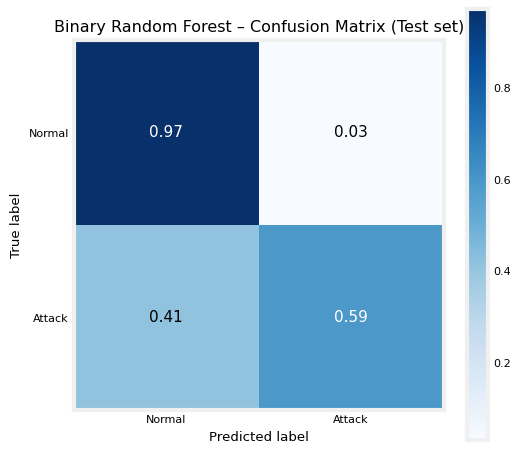
\includegraphics[width=0.7\textwidth]{conf_bin.png}
    \caption{Normalized confusion matrix for binary Logistic Regression}
    \label{fig:binary_lr_cm}
\end{figure}
\FloatBarrier

In addition to the fixed train/validation/test evaluation, stratified 5-fold cross-validation is performed for the binary Logistic Regression baseline. Across folds, the model achieves a mean accuracy of $0.954 \pm 0.001$ and a mean macro-averaged F1-score of $0.950 \pm 0.001$, indicating stable performance across different training subsets under class imbalance.

\subsection{Random Forest}
The Random Forest classifier is evaluated using a reduced feature representation consisting of the top-20 features selected via Random Forest feature-importance scores, as described in Section \ref{sec:models}. This feature subset is used consistently across both binary and multi-class Random Forest experiments. On the binary test set, Random Forest achieves an accuracy of 0.752 and a macro-averaged F1-score of 0.750. Recall is 0.972 for normal traffic and 0.585 for attack traffic. The ROC--AUC on the test set is 0.962. Figure \ref{fig:binary_rf_cm} presents the normalized confusion matrix for the binary Random Forest classifier on the test set.
\begin{figure}[htbp]
    \centering
    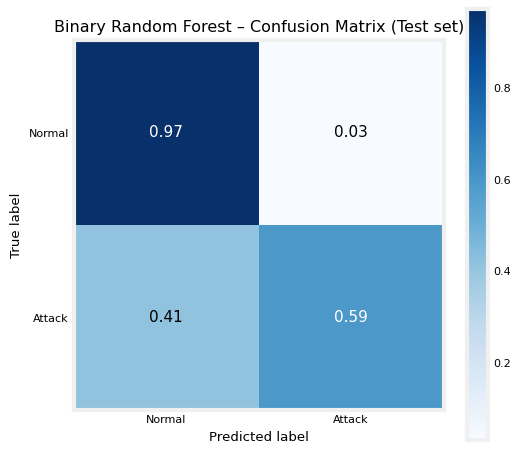
\includegraphics[width=0.7\textwidth]{conf_bin.png} 
    \caption{Normalized confusion matrix for binary Random Forest}
    \label{fig:binary_rf_cm}
\end{figure}
\FloatBarrier

\subsection{Neural Networks}
Although neural networks are not always necessary or consistently superior to classical machine-learning techniques on intrusion-detection datasets, their ability to learn higher-order feature interactions makes them a valuable comparison point. Neural networks are therefore introduced as a third modeling family to assess whether their greater representational capacity provides advantages beyond linear and tree-based methods. On the binary test set, the Neural Network achieves an accuracy of 0.778 and a macro-averaged F1-score of 0.780, with a ROC--AUC of 0.940. Class-specific recall is 0.925 for normal traffic and 0.675 for attack traffic. Figure \ref{fig:binary_nn_cm} shows the normalized confusion matrix for the binary Neural Network on the test set.
\begin{figure}[htbp]
    \centering
    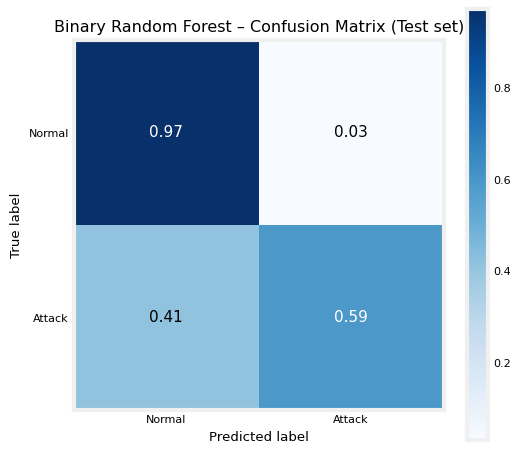
\includegraphics[width=0.7\textwidth]{conf_bin.png}
    \caption{Normalized confusion matrix for binary Neural Network}
    \label{fig:binary_nn_cm}
\end{figure}
\FloatBarrier
\vspace{-1.5em}

\section{Multi-class Classification Results}

In the multi-class setting, models are required to distinguish between normal traffic and four specific attack categories: DoS, Probe, R2L, and U2R. Table \ref{tab:multiclass_results} summarizes the performance of the three models across these categories on the test set.
\begin{table}[htbp]
\centering
\caption{Multi-class classification performance (Recall per class) on the test set.}
\label{tab:multiclass_results}
\begin{tabular}{lccccc}
\toprule
Model & Normal & DoS & Probe & R2L & U2R \\
\midrule
Logistic Regression & 0.934 & 0.811 & 0.655 & 0.046 & 0.160 \\
Random Forest       & 0.972 & 0.793 & 0.748 & 0.044 & 0.010 \\
Neural Network      & 0.925 & 0.776 & 0.702 & 0.165 & 0.700 \\
\bottomrule
\end{tabular}
\end{table}

The results highlight significant differences in how model families handle class imbalance. While Random Forest achieves the highest recall for the majority classes (Normal and Probe), it struggles significantly with the rarest categories, R2L and U2R. In contrast, the Neural Network (specifically Model 3MCv3 with class weighting) demonstrates superior sensitivity to these critical minority attacks, achieving a U2R recall of 0.700, albeit at a slight cost to overall accuracy. Figure \ref{fig:multi_rf_cm} and Figure \ref{fig:multi_nn_cm} present the non-normalized confusion matrices for the Random Forest and Neural Network multi-class models, respectively. These matrices illustrate the absolute error patterns and the models' ability to correctly categorize specific attack types.
\begin{figure}[htbp]
    \centering
    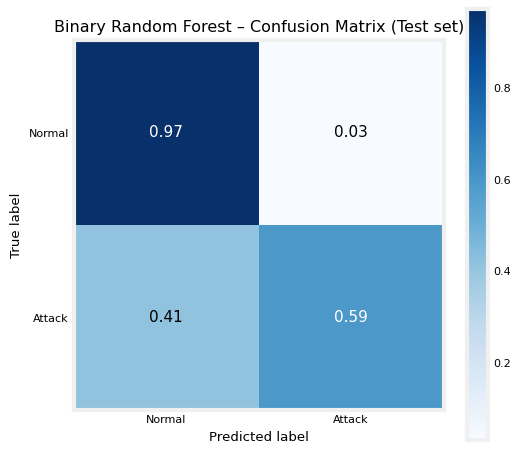
\includegraphics[width=0.7\textwidth]{conf_bin.png}
    \caption{Confusion matrix for multi-class Random Forest}
    \label{fig:multi_rf_cm}
\end{figure}
\FloatBarrier
\vspace{-1.5em}
\begin{figure}[htbp]
    \centering
    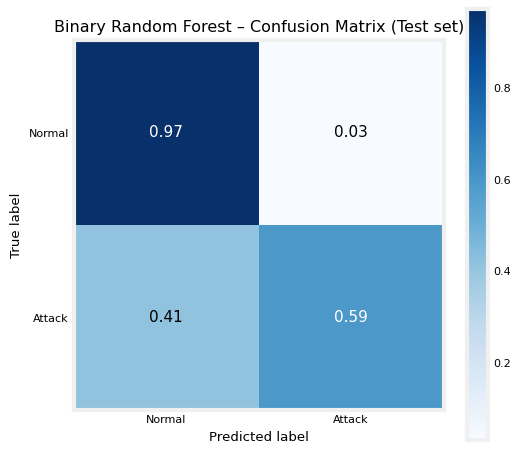
\includegraphics[width=0.7\textwidth]{conf_bin.png}
    \caption{Confusion matrix for multi-class Neural Network}
    \label{fig:multi_nn_cm}
\end{figure}
\FloatBarrier
\vspace{-1.5em}

Overall, the transition from validation to test sets reveals a consistent performance drop across all models, confirming that the NSL-KDD test set contains unseen attack variations that challenge the generalization capabilities of the trained classifiers.